\pagebreak
\section{Microcontroller}

Our microcontroller of choice, the Raspberry Pi 2 Model B, is a preferred choice for embedded robotic systems. One of the deciding factors was the GPIO capabilities on the controller and the interface that it has to offer. It also features a powerful 900MHz quad-core ARM Cortex-A7 CPU and 1 GB of RAM. Because it has an ARMv7 processor, it can run the full range of ARM GNU/Linux distributions\cite{raspispecs}.

\begin{figure}[H]
	\centering
	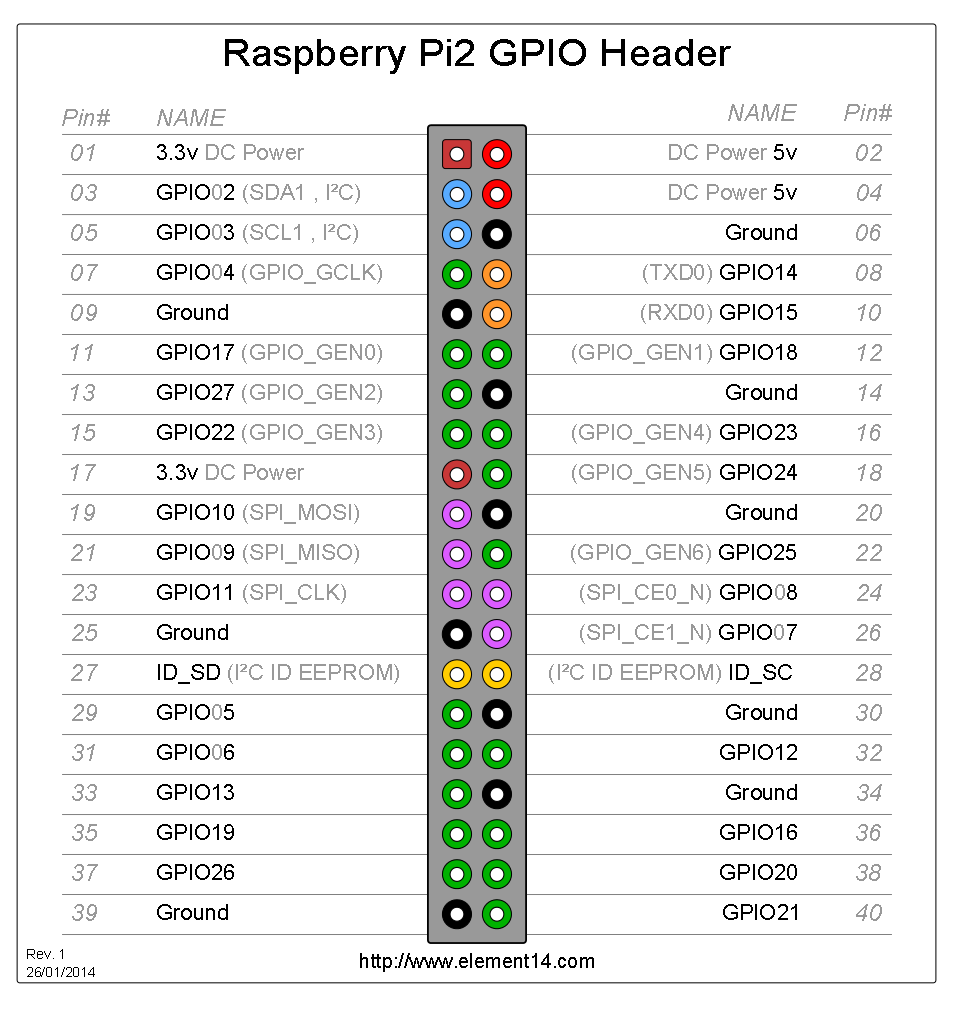
\includegraphics[scale=.4]{images/GPIO_Pi2.png}
	\caption{The pinout of the Raspberry Pi 2 model B, revision 2}
	\label{fig:gpioraspbi2}
\end{figure}

During the initial stages of using ROS we attempted to get the installation up and running on the Raspbian operating system, which is a modified version of the Debian distribution specifically tailored for the Raspberry Pi. The installation was done using the official guide on the Raspberry Pi website\cite{raspiinstall}.

After the installation of the Raspbian operating system, we installed the Indigo distribution of ROS, a Robot Operating System, which is really just a framework for wiring robot software, using their step-by-step guide for the Raspbian operating system\cite{indigoins}.
A source installation had to be done, due to poor support for the Raspbian, and this resulted in an 6-to-8 hour long setup process, because of the need for compiling, building and testing of the whole system. 
During the gathering of the different packages needed for ROS, some unforeseen issues were encountered, like the GMapping package causing issues during installation, since it required Python 2.7.1 and upwards. Through troubleshooting it was then discovered that GMapping package was looking for \textit{Python-2.7.1-0ubuntu2}, instead of the \textit{Python-2.7.3-6+deb7u2} that was installed together with the Raspbian operating system.

Instead of continuing to deal with the ROS issues on the Raspbian operating system, Ubuntu ARM was instead installed on the Raspberry Pi\cite{ubuntuins}.
The installation process using Ubuntu ARM was much faster and more fluent compared to installing ROS on the Raspbian operating system, due to the much broader support for the Ubuntu distribution. The installation only took a couple of hours, by using the built-in package manager, because no installation was required from source\cite{ubuntuROS}.

